\documentclass[a4paper]{article}

% --- Colours (Wong colour-blind-safe palette + cerulean for links) ---
\usepackage{xcolor}
\definecolor{ceruleanblue}{rgb}{0.16, 0.32, 0.75}
\definecolor{wongblue}{rgb}{0.0,0.44705883,0.69803923}
\definecolor{wongyellow}{rgb}{0.9019608,0.62352943,0.0}
\definecolor{wonggreen}{rgb}{0.0,0.61960787,0.4509804}
\definecolor{wongpink}{rgb}{0.8,0.4745098,0.654902}
\definecolor{wonglightblue}{rgb}{0.3372549,0.7058824,0.9137255}
\definecolor{wongorange}{rgb}{0.8352941,0.36862746,0.0}
\definecolor{wonglightyellow}{rgb}{0.9411765,0.89411765,0.25882354}
\colorlet{C0}{wongblue}\colorlet{C1}{wongyellow}\colorlet{C2}{wonggreen}
\colorlet{C3}{wongpink}\colorlet{C4}{wonglightblue}\colorlet{C5}{wongorange}
\colorlet{C6}{wonglightyellow}

\usepackage[colorlinks=true, allcolors=ceruleanblue]{hyperref}
\usepackage[backend=biber, style=phys, eprint=true, sorting=none,
            biblabel=brackets, bibencoding=utf8]{biblatex}
\addbibresource{ref.bib}

\usepackage[margin=2cm]{geometry}
\usepackage{parskip}
\usepackage{graphicx}
\usepackage{subcaption}
\usepackage{booktabs}
\usepackage{placeins}
\captionsetup{labelfont=bf, margin=2cm}
\usepackage{physics}
\usepackage[concrete]{fontsetup}

\title{Auditing a physics-informed augmentation claim:\\
from $+9.8\%$ to a diagnosed negative result}
\author{Simon Krekels}
\date{\today}

\begin{document}
\maketitle

\begin{abstract}
A thermal solar-module classifier reported a $+9.8$ percentage-point accuracy
gain from heat-equation--based synthetic augmentation over a baseline. Under
rigorous evaluation the claim does not survive. Roughly $+9$ points are a
training-schedule artifact (an undertrained baseline); the residual $\sim\!1.9$
points are a \emph{rebalancing} effect that plain image duplication matches or
beats, and they do not improve recall on the rare fault classes the method
targets. Two diagnostics localise the cause: the synthetic images are trivially
separable from real ones (discriminator AUC $0.97$), and class weighting already
handles imbalance more effectively than synthetic rebalancing. A realism upgrade
to the generator, although visually more convincing, measured \emph{worse}
($\text{AUC}\,1.00$). We conclude with the implied redesign: let physics supply
fault \emph{structure} and let a network learn the \emph{appearance}.
\end{abstract}

\section{Setup and metrics}
\begin{itemize}
  \item \textbf{Data.} InfraredSolarModules~\cite{raptormaps2020infrared}:
        $\sim\!20{,}000$ $24\times40$ thermal IR crops, 12 classes, heavily
        imbalanced ($\sim\!50\%$ \texttt{No-Anomaly}; four rare fault classes
        have only $\sim\!120$--$170$ training images each).
  \item \textbf{Model.} EfficientNet-B0~\cite{tan2019efficientnet} fine-tuned
        from ImageNet; inverse-frequency class-weighted cross-entropy;
        warmup\,$\to$\,cosine schedule; stratified $70/15/15$ splits.
  \item \textbf{Harness.} All comparisons are paired on one fixed test set,
        run over 3 seeds, with bootstrap $95\%$ confidence intervals on
        \emph{per-class recall}.
  \item \textbf{Key framing.} The project's objective is \emph{rare-fault
        detection}, so the right metric is \textbf{rare-class recall}, not
        accuracy (which is dominated by the majority class). This distinction
        drives every conclusion below.
\end{itemize}

\section{The headline is mostly a schedule artifact}
The original baseline is undertrained: a slow cosine schedule plus patience-5
early stopping halts it at epoch 12. Fixing only the schedule (a faster 15-epoch
cosine) recovers almost the entire gap with \emph{no} synthetic data
(Table~\ref{tab:schedule}).

\begin{table}[h]\centering
\begin{tabular}{lcc}
\toprule
Run & Schedule & Test acc.\\
\midrule
baseline (as reported)      & 30 ep & 0.690\\
augmented (as reported)     & 30 ep & 0.788\\
clean, retuned schedule     & 15 ep & 0.784\\
augmented, retuned schedule & 15 ep & 0.808\\
\bottomrule
\end{tabular}
\caption{The $+9.8$-point headline is mostly the difference between an
undertrained and a well-trained baseline. A clean model on a 15-epoch schedule
already reaches $0.784$.}
\label{tab:schedule}
\end{table}

\section{The backbone choice holds up}
EfficientNet-B0 is not assumed: it wins a sweep over four \texttt{timm}
backbones on identical clean data, \emph{and} is the smallest. Larger backbones
overfit this small, imbalanced set (Table~\ref{tab:backbone}).

\begin{table}[h]\centering
\begin{tabular}{lccc}
\toprule
Backbone & Params (M) & Test acc. & Macro F1\\
\midrule
\textbf{EfficientNet-B0} & \textbf{4.0} & \textbf{0.784} & \textbf{0.658}\\
MobileNetV3-Large        & 4.2  & 0.760 & 0.646\\
ConvNeXt-Tiny            & 27.8 & 0.745 & 0.635\\
ResNet-50                & 23.5 & 0.694 & 0.577\\
\bottomrule
\end{tabular}
\caption{Backbone sweep (clean data, 15-epoch schedule). Smallest model wins.}
\label{tab:backbone}
\end{table}

\section{Honest baselines: physics is no better than oversampling}
The decisive test compares physics augmentation against the \emph{cheap} ways to
rebalance. \texttt{oversample} duplicates real rare-class images to the same
target count as the synthesiser, isolating the synthetic \emph{signal} from mere
rebalancing; \texttt{randaugment} is a strong generic-augmentation control. We
also toggle class weighting off (``no-weights'') to probe its interaction with
rebalancing (Table~\ref{tab:main}).

\begin{table}[h]\centering
\begin{tabular}{llcccc}
\toprule
Condition & Weights & Acc. & Macro F1 & Macro rec. & \textbf{Rare rec.}\\
\midrule
clean        & yes & 0.782 & 0.658 & 0.699 & \textbf{0.612}\\
oversample   & yes & 0.807 & 0.678 & 0.697 & 0.574\\
randaugment  & yes & 0.782 & 0.654 & 0.702 & 0.615\\
physics      & yes & 0.800 & 0.668 & 0.693 & 0.569\\
\midrule
clean        & no  & 0.839 & 0.699 & 0.684 & 0.560\\
oversample   & no  & 0.826 & 0.685 & 0.680 & 0.582\\
physics      & no  & 0.837 & 0.700 & 0.686 & 0.568\\
\bottomrule
\end{tabular}
\caption{Honest baselines, 15-epoch schedule, 3-seed means. Physics is
statistically indistinguishable from \texttt{oversample} on every metric, and is
the \emph{worst} condition on rare-class recall.}
\label{tab:main}
\end{table}

Findings:
\begin{itemize}
  \item \textbf{Physics does not beat duplication.} On accuracy, \texttt{oversample}
        ($0.807$) edges out \texttt{physics} ($0.800$); elsewhere they are within
        noise. The synthetic pixels add nothing over copy-paste.
  \item \textbf{The accuracy gain is a rebalancing artifact, not rare-fault
        improvement.} Physics' $+1.9$ points over \texttt{clean} (3-seed paired
        $+0.019\pm0.006$) come from the \emph{majority} class
        (\texttt{No-Anomaly} recall $0.85\!\to\!0.88$); on rare-class recall
        physics is worst, and significantly below \texttt{clean} (paired
        $\Delta=+0.043$, $95\%$ CI $[0.003,0.082]$). See
        Fig.~\ref{fig:rare}.
  \item \textbf{Class weighting is the strongest single lever for rare classes.}
        \texttt{clean} with weights ($0.612$) beats every other condition.
        Turning weights off trades rare recall for accuracy ($0.78\!\to\!0.84$).
        Data rebalancing is a weaker \emph{substitute} that \emph{hurts} when
        stacked on weighting --- exactly the current configuration.
\end{itemize}

\begin{figure}[h]\centering
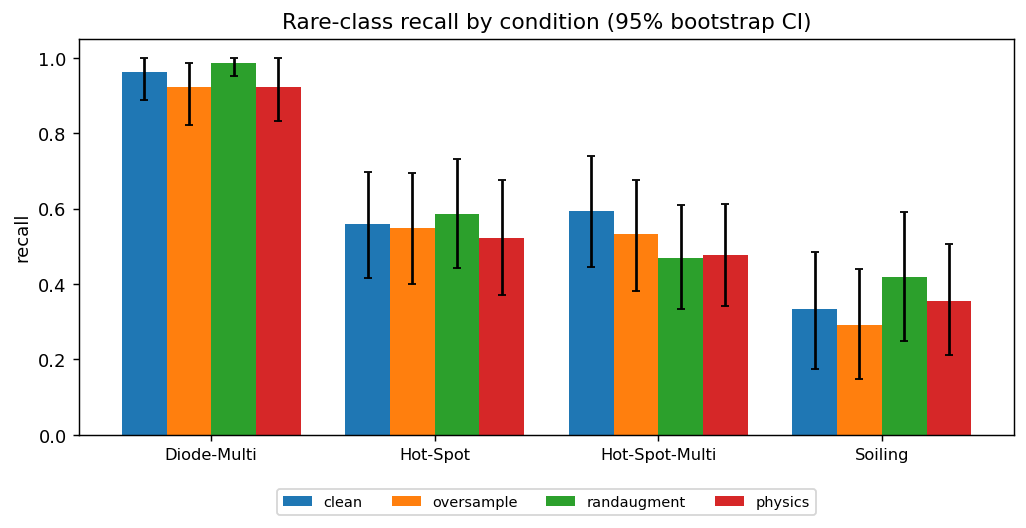
\includegraphics[width=0.92\linewidth]{fig_rare_recall.png}
\caption{Rare-class recall with $95\%$ bootstrap CIs. Physics (red) is never the
best bar. Wide intervals (each rare class has $\sim\!25$ test images) are
themselves a finding: the evaluation is underpowered, which is why a
metric-appropriate, CI-based harness was necessary.}
\label{fig:rare}
\end{figure}

\section{Diagnostics: why it fails}
Two cheap diagnostics localise the failure to \emph{two independent} causes.

\textbf{D1 --- domain gap (Fig.~\ref{fig:auc}).} A classifier separates synthetic
from real images of the same classes at AUC $0.966$. The gap survives heavy
low-pass blurring ($0.934$ at radius 2, $0.867$ at radius 4), so it lives in the
\emph{coarse shape} of the steady-state heat blobs, not in seams or compression:
the synthetic faults simply do not look like real faults.

\textbf{D2 --- redundant rebalancing.} The ``no-weights'' rows of
Table~\ref{tab:main} confirm that class weighting and data rebalancing are
\emph{substitutes} for handling imbalance; stacking them over-corrects toward the
majority and lowers rare recall. Even a perfect synthesiser would have to be
deployed without fighting the class weights.

\begin{figure}[h]\centering
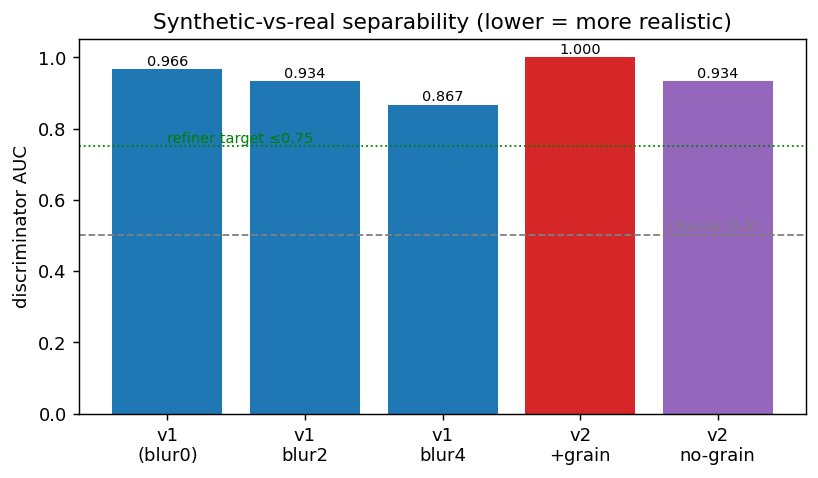
\includegraphics[width=0.7\linewidth]{fig_d1_auc.png}
\caption{Synthetic-vs-real discriminator AUC (lower is more realistic). The v2
realism upgrade made the gap \emph{worse}.}
\label{fig:auc}
\end{figure}

\FloatBarrier
\section{A realism upgrade that measured worse (v2)}
A second generator (\texttt{heat\_equation\_v2}) replaced steady-state blobs with
\emph{transient} diffusion, fixed an aspect-ratio warp, calibrated per-class
contrast to real data, and corrected the class models (real ``Soiling'' is bright
and streaky, not a smooth darkening). It looks markedly more realistic
(Fig.~\ref{fig:montage}) --- yet the discriminator scored it \emph{worse}: AUC
$1.000$ with the (na\"ively added, i.i.d.) sensor grain, and $0.934$ once the
grain was ablated. Lessons:
\begin{itemize}
  \item \textbf{Visual realism is misleading;} the objective discriminator is the
        right judge. Adding i.i.d.\ grain on top of a base that already carries
        real, spatially-correlated noise is an obvious tell.
  \item \textbf{The additive-blend-on-clean-base paradigm is near a detectability
        ceiling:} corrected, v2 ($0.934$) is no better than v1 ($0.966$).
        Incremental geometry tweaks will not close the gap.
\end{itemize}

\begin{figure}[h]\centering
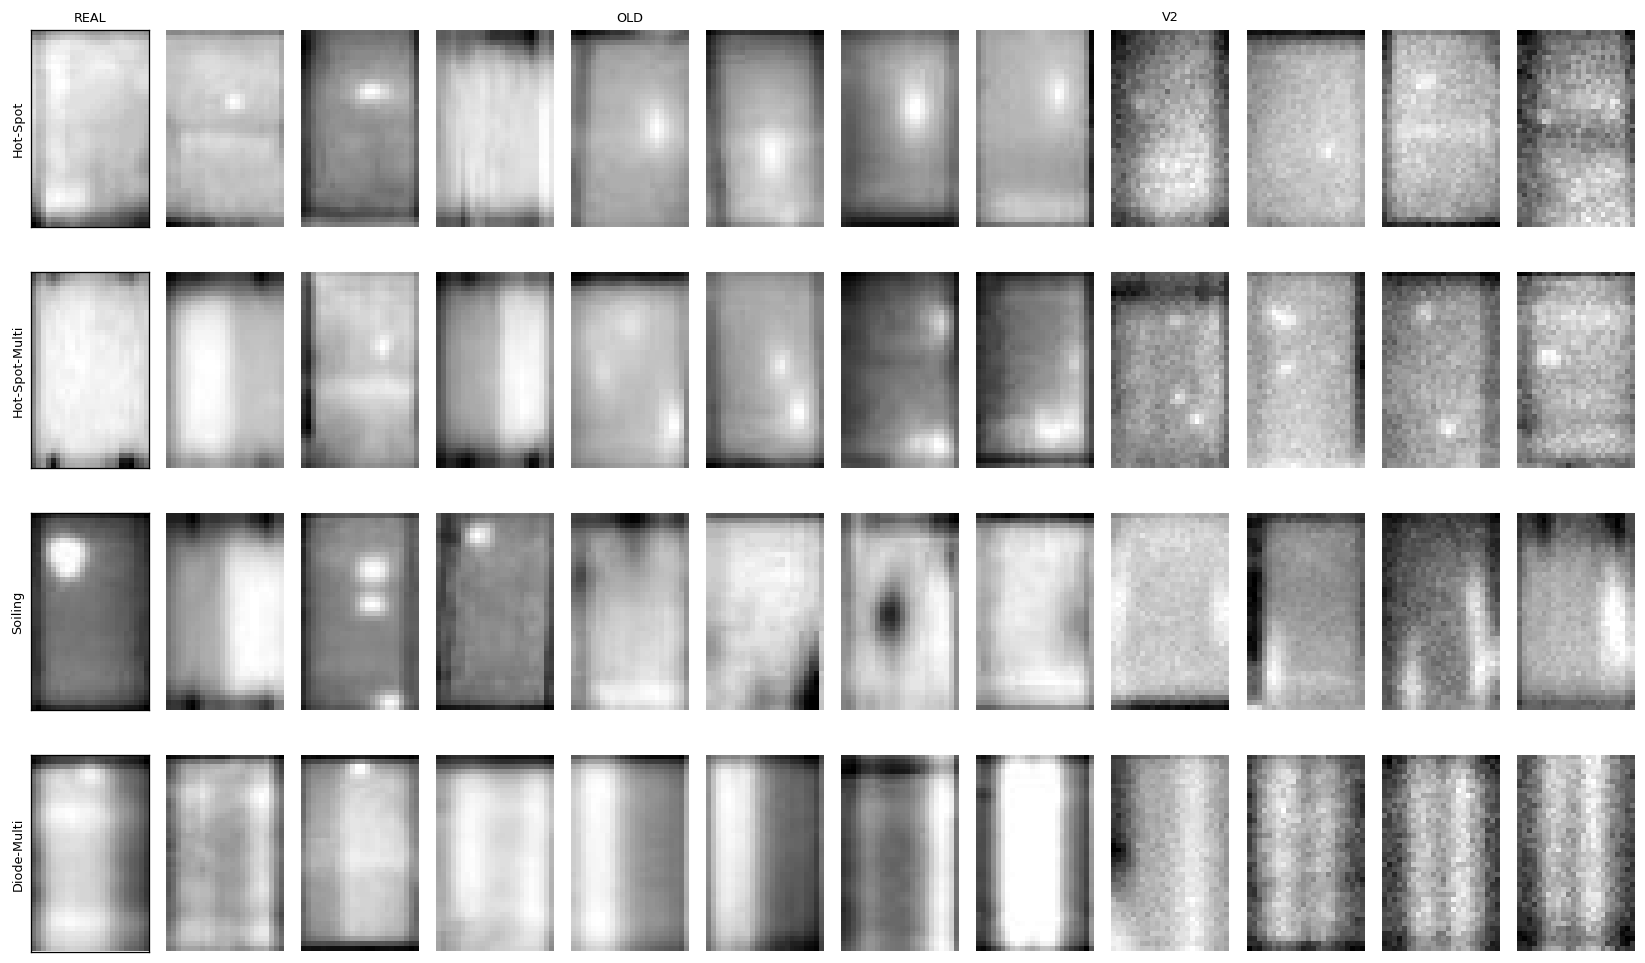
\includegraphics[width=\linewidth]{montage_v2.png}
\caption{Real $\mid$ v1-synthetic $\mid$ v2-synthetic for the four augmented
classes. v2 is visually closer, but measured more separable --- the cautionary
core of this report.}
\label{fig:montage}
\end{figure}

\FloatBarrier
\section{Discussion: the right role for physics}
The error was asking physics to generate \emph{pixels}. A hand-specified PDE is
good at \emph{structure} (where heat is, how it diffuses --- which carries the
label) and bad at \emph{appearance} (sensor texture, noise statistics, tone
mapping). The defensible division of labour is therefore: \textbf{physics
proposes the fault structure; a learned model renders the appearance.} This keeps
physics genuinely load-bearing rather than decorative, and turns the realism gap
into a learning target instead of a hand-tuning chore.

\section{Future work: a learned refiner (SimGAN)}
\label{sec:future}
We propose a SimGAN-style refiner~\cite{shrivastava2017simgan}: a small
fully-convolutional residual network $R$ takes a physics-generated image and
outputs a more realistic one, trained adversarially against a patch discriminator
\emph{plus} a self-regularization term $\lambda\norm{R(x)-x}_1$ that preserves the
physics-determined fault (hence the label). The discriminator already built for
D1 doubles as both the adversary and --- crucially, with an \emph{independently
trained} copy --- the scorecard.

Validation is staged and honestly gated:
\begin{enumerate}
  \item \textbf{Realism gate.} Refine the synthetic set and re-score with a fresh
        discriminator. Success: AUC falls from $0.93$ toward $\le 0.75$.
  \item \textbf{Utility gate} (only if the first passes). Add a
        \texttt{physics\_refined} condition to the harness and test rare-class
        recall against \texttt{oversample}, with weights off (per D2). Success:
        a positive paired delta whose CI excludes zero.
\end{enumerate}
Because the heat solver is a stack of Laplacian convolutions --- a fixed-weight
CNN --- the entire pipeline is differentiable, enabling a later variant that
learns the source field or PDE parameters end-to-end through the physics. The
binding constraints remain: $\sim\!600$ real fault images is a tight data budget,
and any generator must clear \emph{both} gates, not just the first. If the realism
gate fails, the negative result documented here stands --- which is itself an
acceptable, well-characterised outcome.

\printbibliography
\end{document}
